\documentclass{article}
\usepackage[top=1in, bottom=1in, left=1in, right=1in]{geometry}
\usepackage{url}
\usepackage{fancyhdr}
\pagestyle{fancy}
\usepackage{setspace}
\onehalfspacing
\usepackage{graphicx}

\lhead{Building a Reliable ISP}
\rhead{Doug Woos and Qiao Zhang}

\begin{document}

\section{Introduction}

The modern Internet is deficient in reliability, security,
customizability and evolvability. The main problem is that ISPs cannot
control end-to-end deliverability of their customers' packets or
independently introduce new services. Under the constraint of ISPs
only being able to provide what they can guarantee themselves, our
broad goal is enable ISPs to provide reliable packet delivery from one
end-host to another and a bundle of other crucial services to their
customers. However, the first obstacle is that ISPs are currently
constrained by the design of using routers and switches with
proprietary ASICs and outmoded routing protocols. Our next step is
therefore to design an ISP that is more reliable and agile.

In our model, a client will make a contract with an ISP to obtain
specific guarantees about packets it sends through that ISPs
network. Specifically, the ISP agrees to deliver packets from one
specific Point of Presence (PoP) to another. The ingress PoP could
either be the client's location or that of some other ISP with which
the client has negotiated a service contract; similarly, the egress PoP
could be either the final destination for the client's traffic or some
other ISP. The crucial point is that from the ISP's perspective, it
\textbf{does not matter}. The contract it has made with the client
provides delivery guarantees only between the ingress PoP and the
egress PoP. Examples of the guarantees the ISP could provide include
promises about uptime, bandwidth, and latency; for instance, Reliable
Transit Inc. might promise the client 100 Mb/s from PoP A to PoP B
with 99.999\% of uptime, with a latency between 50 and 100 ms. The client
is then responsible for stitching together a route between such ISPs.

Our goal is to implement an ISP that is capable of making such
promises to clients and reliably routing traffic according to the SLA. Clients can
communicate with the ISP on the control plane and the data plane. The
control plane is used to create a contract with the ISP; a client
requests a route from PoP A to PoP B and the ISP responds with a token
that the client can attach to packets so that the ISP knows to send
them along that route. The data plane is used to forward the
packets. If a packet arrives at the ingress PoP with a token the ISP
recognizes, the ISP is responsible for routing that token to the
egress PoP.

The primary challenge in implementing such an ISP is
fault-tolerance. Traditional ISPs are configured using the BGP
protocol for inter-domain routing, which provides edge routers with information about what the
next hop should be for a given destination IP address. BGP routing updates are known to
propagate slowly. In contrast, our ISP needs to
configure its edge routers dynamically to provide a route servicing
each new contract. The circuit state or the mapping from client circuit tokens to
routes needs to be propagated and stored at the edge nodes in a
fault-tolerant manner so that if an edge node fails the remaining
nodes are able to route client traffic correctly. If there is a
failure at an edge node, neighboring ISPs must cooperate to route
around the failing node. Thus, we introduce a simple failover
protocol. Our failovers are initiated on the client side since we believe the
client is best positioned to detect failures in the path and should be left to
decide how often to check for failed deliveries or what
an appropriate delivery timeout looks like.

Our primary contributions are:
\begin{enumerate}
\item A proof-of-concept implementation of a fault-tolerant
  inter-domain routing system,
\item The circuit establishment protocol,
\item The failover protocol.
\end{enumerate}

\section{Related Work}
Our work is an implementation of the model presented in the Transit as
a Service (TaaS) paper \cite{taas}. In the TaaS model, there are two
types of principals: end-hosts and ISPs. When end-host \texttt{A}
wants to establish a circuit to end-host \texttt{B}, it uses an internet
atlas service such as iPlane \cite{iplane} to find a route to
\texttt{B} which goes through one or more TaaS-supporting ISPs. It
then contacts these ISPs individually and purchases service from each
of them. This service comes with a service level agreement (SLA) which can
provide guarantees about latency, bandwidth, uptime, and even
security. Once the client has purchased service from each ISP on the
route, it can send traffic through the newly-established circuit and
be confident that its traffic will be delivered consistently and in a
timely fashion. The TaaS paper provided a simulation of traffic
flowing through reliable ISPs, but did not actually implement such an
ISP. Our contribution is to provide a working, proof-of-concept
implementation of a reliable TaaS-supporting ISP, and to show that it
is possible to get adequate performance and reliability.

The problem TaaS seeks to solve--the poor reliability and security of
current inter-domain routing technologies--is quite apparent, and
there have been many other attempts to improve the situation. Systems
like Pathlet routing \cite{pathlet}, Icing \cite{icing}, and SCION
\cite{scion} are similar to TaaS in that they give end-hosts more
control over the path their packets will take. Each of these, however,
involves a more fundamental redesign of the Internet than the small
changes proposed by TaaS. TaaS can operate over existing connections
and using existing protocols, only requiring changes at the edges of
ISPs wishing to provide TaaS services.

Another area of related work is in Software Defined
Networking. Systems like Frenetic \cite{frenetic} allow users to
dynamically configure switches and define routes through the network
dynamically. TaaS provides a similar flexibility for the internet as a
whole; clients can view each ISP as a switch, which will reliably
route traffic from one location to another. By stitching together a
series of these ISPs, a client can be confident that its packets will
arrive at an end-host reliably and promptly.

\section{Architecture Overview}
\begin{figure}
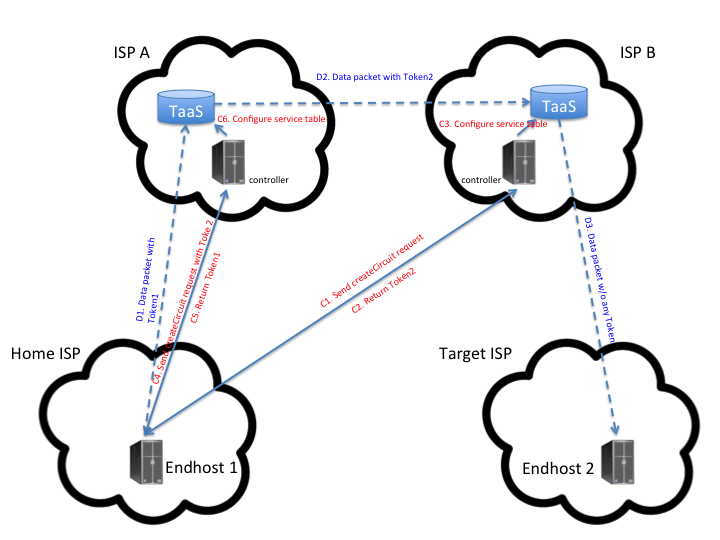
\includegraphics[width=\linewidth]{diagram}
\caption{Architecture Diagram}
\label{fig:diagram}
\end{figure}

We first describe the control plane and data plane of our ISP that
allow clients to establish circuits at various ISPs and stitch
together path segments from each ISP to forward their traffic reliably
to other end-hosts. We then describe how each ISP can maintain circuit
states in a fault-tolerant fashion. Our architecture supports an
overlay network over the IP layer that guarantees reliable end-to-end
packet delivery.

\subsection{Control Plane}

The clients can find out the costs and network guarantees provided by
a TaaS-supporting ISP through an iPlane-like service (for this
project, we assume that this is available and therefore will not
implement it). Each ISP PoP has controllers that receive requests from
clients to establish intra-domain circuits. On receiving a
createCircuit request (C1 in Figure \ref{fig:diagram}), the
controllers respond with a per-circuit-per-client authentication token
(C2) to the client. The controllers subsequently update the forwarding
tables of the edge nodes (C3) to add the new forwarding rules in there.
The same sequence of events (C4, C5, C6) happen at every ISP in the
circuit that the client contacts.

At the end of the circuit establishment phase, every ISP on the
end-to-end path will have configured its data plane to have the
appropriate forwarding rules in their forwarding tables. The clients
will have a token for every circuit at every ISP that it makes
contracts with. However, since ISPs use client tokens to identify
circuits for incoming data packets, in order for clients to stitch
together circuits from different ISPs to form one end-to-end path, the
packet either has to carry all the tokens for every circuit along the
path, or the token on the packet gets modified as it exits from one
ISP and enter the next one. We adopt the second approach, and
consequently, each ISP also needs to remember the token for the next
path segment for another ISP. The createCircuit request from the
client therefore needs to contain the token for the next path
segment. The client thus needs to establish the whole path starting from
the last path segment entering target ISP to the first path segment
exiting the home ISP, as shown in Figure \ref{fig:diagram}, and the
ordering is conveyed by the sequence number of the control plane messages
(C1, C2, ..., C6). More details can be found in the TaaS paper.

\subsection{Data Plane and Stateful transformation of packets}

In order to enable each PoP to route packets through the circuit the
client purchased, we insert a TaaS-aware Serval layer in each
packet. The TaaS/Serval layer sits on top of the IP layer and below
the transport layer in the network protocol stack. The Serval header
will contain the client token that identifies the intended circuit
within the ISP. The end-hosts and each of the PoPs in a TaaS-supported
ISP will be running Serval module which allows the packet to be
transformed as it is being routed through the circuit, e.g. the PoPs
modifies the destination IP address and TaaS token of the packet as it
is routed from one hop to another. For example, as shown in Fig. \ref{fig:diagram},
 the client (End-host 1), having established the path,
 sends data packets with Token1 to ISP A. The edge nodes at
ISP A use Token1 to identify the circuit the client has purchased and
forward the packets to ISP B, while changing the token to Token2. On
receiving the packet identified by Token2, ISP B routes the packet to
the Target ISP, stripping the TaaS token as the packet exits its
network.

Our ISP needs to maintain the circuit states at the control plane in a
fault-tolerant fashion. When a client requests and establishes a
circuit with any controller, we need to update and replicate the
circuit state at a group of designated nodes at the PoP. This is
coordinated using Apache
Zookeeper\footnote{\url{http://zookeeper.apache.org/}}, an open-source
distributed coordination service. It ensures that a majority of those
designated nodes are aware of any given route through the system;
thus, if a node fails, the client can send traffic through a different
node. The main weakness of Paxos is its performance cost, but as these
operations are restricted to the control plane, there is no need for
them to be especially fast (clients will send data through the system
far more often than they will request new routes).

\subsection{Failover}

In our system, failures can potentially occur at several different
levels:

\begin{enumerate}
\item Failure of a whole ISP
\item Failure of a core node
\item Failure of an edge node
\end{enumerate}

If the ISP as a whole fails, the client will need to discover this and
either provision an alternate route to its end-host or accept that its
traffic will not get through until the failed ISP comes back
online. If the client chooses to route around the failed ISP, it will
need to initiate the TaaS circuit construction protocol again, this
time ensuring that it does not purchase service from the failed ISP.

If a core node fails, the ISP is responsible for detecting this
failure and routing around it. There are many established systems for
doing so; one recent example is Data-Driven Connectivity \cite{ddc},
in which packets which cannot be delivered due to failure are bounced
back up the path they came down until another path can be
established. Each ISP can choose to recover from these internal
failures by whatever method it chooses so long as its SLAs are
maintained.

The last failover case is failure at an edge node. Since edge nodes
correspond to boundaries between ISPs, edge nodes belonging to
different ISPs need to cooperatively handle failover; thus, we have
designed a failover protocol which must be implemented by each
participating ISP.  Our system does not perform failure detection,
since we believe that in general the client will be able to do a
better job of determining whether its traffic is actually arriving at
the server. Therefore, failover is a client-driven process. When the
client detects a failover (i.e. it detects that its traffic is not
successfully arriving at the server), it notifies the first ISP that
it believes a problem has occured. If it does not receive an
acknowledgment from the first ISP, it concludes that that is where the
failure exists and fails over to another edge node in the same ISP. If
the first ISP does receive the client's message, it first acknowledges
it so that the client doesn't assume it has failed, then checks the
second ISP in the same way that the client checked it. Thus, the
process is initiated by the client but is actually performed at each
non-failing ISP node in the circuit.

For example, assume a circuit has been established between a client C,
ISP A, ISP B, and a server S. Each ISP has 3 routing nodes; we call
them A1, A2, A3 and B1, B2, B3. When the circuit is first established,
it goes from C to A1 to B1 to S. At some later time, B1 fails. C
detects that S isn't receiving its messages (perhaps it isn't getting
acknowledgments back). C initiates the failover process by sending a
message to A1. A1 receives and acknowledges this message, then sends a
message to B1. A1 never receives an acknowledgment, and concludes
(correctly) that B1 has failed. A1 then sends a message to B2, which
acknowledges it. A1 updates its local state so that packets on the
circuit go to B2 rather than B1, then informs the client that the
failover has succeeded. Subsequent traffic is now routed through the
new circuit.

\section{Implementation}
\subsection{Control plane}
We implemented the control plane (circuit establishment and failover)
as daemons written in the Python programming language. The client
communicates with these daemons using protocol
buffers\footnote{\url{https://code.google.com/p/protobuf/}}, an open
standard for binary message serialization. A third daemon runs on each
ISP edge node and ensures that its local routing state (described in
the next section) corresponds to the state in Zookeeper.
\subsection{Data plane}
As a proof of concept, we implemented our design as an overlay on top
of the IP layer using Serval, a service-oriented networking system. On
each node, Serval keeps a service table, which is a mapping from
integer service IDs to rules. These rules can either be demux rules
which correspond to Serval sockets opened by local applications or
forwarding rules. A forwarding rule contains the IP address of another
machine running Serval.

A Serval packet has an extra header (inside the IP header but wrapping
the layer 3 header) which contains its destination service ID. When
Serval sees an incoming packet, it looks up the packet's service ID in
its local table. If it finds a demux rule, it places the packet on
the corrsponding local socket's queue and notifies the application
which owns the socket. If it finds a forwarding rule, it forwards the
packet on to the corresponding IP address.

\begin{table}
\centering
\begin{tabular}{| l | l | l | l | }
  \hline
  ISP & Service ID & TaaS Auth & IP \\ \hline
  ISP1 & auth1 & auth2 & ISP2 \\ \hline
  ISP1 & auth2 & auth3 & ISP3 \\ \hline
\end{tabular}
\caption{ISP service tables}
\label{table:servicetables}
\end{table}

We modified Serval to add an extra field to forwarding rules and
Serval headers which corresponds to the TaaS authenticator. When our
modified version of Serval receives a request which contains a TaaS
authenticator, it uses that authenticator instead of the incoming
service ID to find the packet's destination. For instance, if the
service tables are configured as in Table \ref{table:servicetables},
when ISP1 sees an incoming packet with TaaS authenticator
\texttt{auth1}, it looks it up in its service table and finds the
entry for ISP2. It then updates the packet's Serval header so that its
TaaS authenticator field is \texttt{auth2} and forwards the packet to
ISP2. ISP2 then does the same process and forwards the packet to
ISP3. Thus a packet is routed through the system base on a series of
authenticators, where each authenticator is defined by one ISP and
used by another.

\begin{table}
\centering
\begin{tabular}{| l | l | l | }
  \hline
  Service ID & TaaS Auth & IP \\ \hline
  id1 & auth1 & ISP1 \\ \hline
\end{tabular}
\caption{Client service table}
\label{table:clientservice}
\end{table}

Serval has a system for ``translating'' IP traffic to serval traffic
so that both the client and server can use standard IP sockets and the
intermediate nodes (ISP nodes in our case) can run
Serval. Unfortunately, we were unable to get this system
working. Therefore, we require the client and the server to run Serval
as well. The client's service table will include a service matching
Table \ref{table:clientservice}. \texttt{id1} is defined by the
client; any application on the client which wants to use the circuit
should open a Serval socket on \texttt{id1}. Packets sent on that
socket will include \texttt{auth1} as the authenticator, which ISP1
will use to find its entry for the circuit.

\section{Evaluation}

We deploy our ISP PoPs on the VICCI testbed.
Ideally, we want each VICCI site to function
as a PoP to simulate the geographical spread of ISP PoPs.
However, due to uncooperative network interfaces on VICCI nodes,
Serval has problems delivering packets across VICCI clusters.
As a result, we have to deploy all three ISPs within a single VICCI cluster,
 the University of Washington (UW) cluster. The clients and servers are also deployed
 on the UW cluster.
For each ISP PoP, we set up
one node to be the TaaS control plane that clients establish circuits with
and three nodes to be the TaaS data plane that forwards
traffic. The coordination service provided by Zookeeper is hosted
at a separate node from control plane or data plane that maintains consistency
in the circuit state within a PoP.

There are two goals in our evaluation. The first goal is to establish
the feasibility of stateful transformation in our ISPs. We
deploy our ISP infrastructures on VICCI nodes and have O(100)
clients establish circuits through our ISPs. We use simple UDP clients
and UDP echo servers to verify that our infrastructure can deliver packets
using the path the clients established.

The second goal is to evaluate the fault-tolerance of our ISPs and test
our failover protocols.
 Within each ISP, the state (the mapping from client token to the circuit the
client purchased) maintained at each PoP needs to be resilient to
failures. We arbitrarily shut down the second ISP edge nodes one at a time,
 and then measure the failover time for the path to recover from failures.

In our experiment, we first establish an end-to-end path from the client
to the server via 3 ISP PoPs using our control plane infrastructure.
Then, we obtain three sets of measurements, where
 $5, 20$ and $40$ UDP clients talk to the corresponding
number of UDP echo servers using the path we just established, and
we attempt to measure the failover time versus the number of clients
sharing the path.
In each measurement, all the UDP clients can successfully receive
the echoes from the servers. This establishes the feasibility of
stateful transformation in our ISP under mild workload.
In order to trigger failover, we shutdown the network interface of the
nodes in the data plane at ISP 2. The clients can successfully detect
the failures in the path through timeout (we expect applications will
have reasonable ways of figuring out path failures). The clients then
send check-failover requests to the failover daemons running on the
ISP data plane. Our failover daemons successfully run the failover
protocol and measurements of the failover time is shown in Fig. \ref{fig:failover}.

\begin{figure}
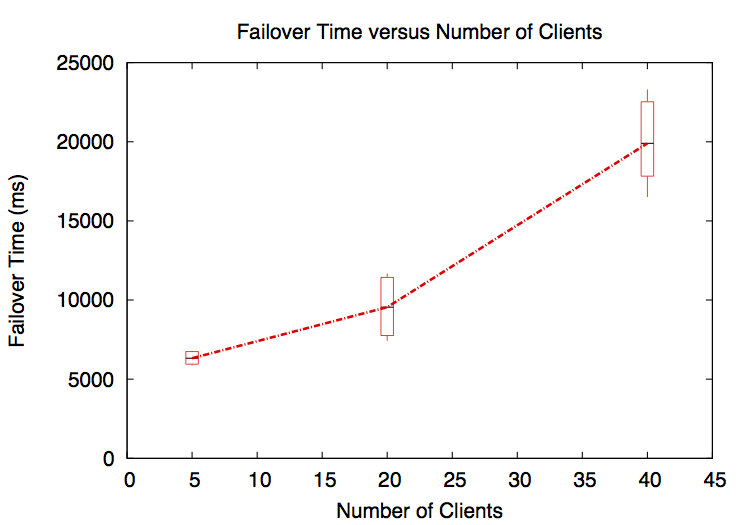
\includegraphics[width=\linewidth]{failoverTime_numClients}
\caption{A Plot of Failover Time vs. Number of Clients}
\label{fig:failover}
\end{figure}

Fig. \ref{fig:failover} shows the failover time versus the number of clients
measurements. We make a few main observations:
\begin{enumerate}
\item for workloads sharing the same path, the failover time for a
  single ISP edge node failure using our infrastructure is tens of
  seconds, in contrast to a failover time on the order of hours or
  even days using BGP;
\item the failover time increases with the number of applications
  sharing the path;
\item the variability of failover time also increases as the number of
  application sharing the path increases.
\end{enumerate}

We can conclude from our experiments that reliable ISPs can feasibly
provide transit to numerous clients, and can respond to failures in a
reasonably short time (seconds, as opposed to hours or even days with
current protocols).

\section{Future Work}

Our three ISPs are all hosted on the UW VICCI cluster due to network
interface issues with VICCI. We will need to conduct future
experiments and find out if a more long haul network would
significantly increase the failover time.

Despite the feasibility of executing failover, our infrastructure is
not optimized for efficiency. The bottleneck in the failover time is
due to the significant delays in having zookeeper propagating circuit
states and updating the Serval service table on the data plane. We
envision more fine-grained updates to the circuit states will
significantly shorten the failover time.

Due to difficulties in maintaining a large number of usable VICCI
nodes, we limit ourselves to only simulate the most interesting
failures cases. We did not simulate failures at the circuit
establishment nodes or the Zookeeper nodes. On a more full scale
evaluation, we can potentially simulate those failure cases too.

We did not measure the routing performance of our ISPs. A more
extensive evaluation can include those performance metrics.

Our ISP infrastructure can be extended to provide a range of services,
in addition to provisioning a path for the clients. We envision that
clients can obtain guarantees for Quality of Service, bandwidth and
other useful services that an ISP can provide.

\section{Conclusion}
Deficient interdomain routing protocols are responsible for many of
the modern internet's fundamental reliability, performance, and
security issues. When an end-host sends a packet out--a packet which
might contain an email to a friend, crucial health monitoring data, or
national secrets--the end-host has very little control over the path
this packet will traverse through the internet before arriving--or
not--at its intended destination. We seek to remedy this issue by
allowing end-hosts to purchase service from reliable, fault-tolerant
ISPs, stitching together a sequence of such ISPs to provide a
reliable, secure, and fast path through the internet.

Our contribution is a working, proof-of-concept implementation of a
reliable and fault-tolerant ISP, including protocols for circuit
establishment and failover. We describe the architecture and
implementation of an individual ISP, and evaluate the performance of a
complete circuit.

\bibliography{bibliography}
\bibliographystyle{plain}

\end{document}
